\documentclass[conference]{IEEEtran}
\usepackage[T1]{fontenc}
\usepackage[utf8]{inputenc}
\usepackage{cite}
\usepackage{amsmath}
\usepackage{graphicx}
\usepackage{float}
\usepackage{stfloats}
\usepackage{booktabs,longtable,array,tabularx}
\usepackage[hidelinks]{hyperref}
\hypersetup{pdftitle={Evaluation of RGB, Depth, and RGB-D Methods for
Low-Lying Obstacle Detection in Indoor Robot
Navigation},pdfauthor={Jakub Dusza; Juan Gómez-Elvira Carrocera}}
\providecommand{\tightlist}{\setlength{\itemsep}{0pt}\setlength{\parskip}{0pt}}

\graphicspath{{figures/}}
\begin{document}
\title{Evaluation of RGB, Depth, and RGB-D Methods for Low-Lying
Obstacle Detection in Indoor Robot Navigation}
\author{\IEEEauthorblockN{Jakub Dusza}\and \IEEEauthorblockN{Juan
Gómez-Elvira Carrocera}}
\maketitle
\raggedbottom

\section{Introduction}\label{i.-introduction}

Safe navigation in indoor environments requires mobile robots to detect
not only large obstacles such as walls and furniture, but also small and
low-lying objects such as cables, latex gloves, screws, and other
floor-level hazards. These obstacles are particularly challenging
because they occupy few pixels in images captured by the robot's camera
and may also be difficult to distinguish from the floor using depth
sensors. Previous work has therefore explored both appearance-based
methods using RGB images and geometric methods using depth or RGB-D
information. Hua et al.~\cite{hua2019small} showed that combining RGB
and depth information can improve small-obstacle segmentation for
robotic navigation, although the obstacles considered in their
experiments were generally larger than thin or flat objects such as
cables or screws.

The objective of this project is to evaluate methods for detecting thin
and low-lying indoor obstacles, with particular emphasis on the
contribution of RGB and stereo-depth information. The methods are
evaluated using the Indoor Small Objects Dataset (ISOD), introduced by
Chen et al.~\cite{chen2023self}, which provides aligned RGB and depth
data together with binary semantic segmentation labels for floor scenes
containing objects typically no higher than 3 cm. The comparison uses
ESANet \cite{seichter2021efficient} with RGB, depth and RGB-D inputs,
alongside RGB models U-Net \cite{ronneberger2015u} and
YOLOv8n-seg\footnote{\url{https://docs.ultralytics.com/tasks/segment/}},
and a depth-only floor-plane baseline. The methods are also tested on
our GTE-Floor recordings acquired with the robot's camera. We
additionally test whether automatic training masks from SAM 3
\cite{carion2026sam} can reduce manual annotation without reducing
obstacle-detection performance.

\section{State of the Art}\label{ii.-state-of-the-art}

Hua et al.~\cite{hua2019small} proposed a two-stage RGB-D semantic
segmentation system for small-obstacle avoidance. The first stage
identifies the traversable road or floor region, while the second stage
detects obstacles inside this region. Separate RGB and depth branches
are used to extract and combine visual and geometric information. Their
work demonstrates the usefulness of RGB-D sensing for obstacle
perception, but their custom dataset contains obstacles measuring at
least 5 cm in each dimension, larger than floor-level hazards such as
cables.

Chen et al.~\cite{chen2023self} proposed MOSTS, a lightweight one-shot
texture segmentation model for indoor robot navigation. Their system
first estimates the ground plane from depth, point-cloud, and IMU
information using filtering, RANSAC, and PCA, and then applies RGB
texture segmentation to identify traversable floor regions. The authors
report that their geometric ground-plane method typically detects
objects higher than approximately 5 cm, meaning that objects closer to
the floor may be missed by depth sensing. MOSTS addresses this
limitation by comparing a query image with a reference image of the
desired floor texture. On ISOD, MOSTS with a MobileNetV3 backbone
achieves 85.7\% mean intersection over union (mIoU) for drivable-area
segmentation while remaining suitable for real-time operation. However,
its dependence on a reference floor texture may reduce robustness when
several valid floor appearances occur in the same environment. The
authors use ISOD for validation; our project instead trains on part of
this dataset and evaluates obstacle masks, so the scores measure
different tasks.

RedNet, proposed by Jiang et al.~\cite{jiang2018rednet}, and ESANet,
introduced by Seichter et al.~\cite{seichter2021efficient}, provide
RGB-D fusion approaches benchmarked in the MOSTS paper. RedNet extracts
RGB and depth features in separate encoders and combines them at several
stages. ESANet uses attention to weight and combine features from its
RGB and depth encoders. Its published RGB-only, depth-only and RGB-D
versions let us compare the three inputs within one model family.

Semantic segmentation architectures provide another direct approach to
the problem because they classify each image pixel rather than requiring
individual obstacle instances. SegNet \cite{badrinarayanan2017segnet}
uses an encoder-decoder architecture in which pooling indices from the
encoder are reused during upsampling, providing an efficient approach to
pixel-wise semantic segmentation. DeepLabV3+ \cite{chen2018encoder}
combines atrous spatial pyramid pooling with an encoder-decoder
architecture to capture multi-scale contextual information while
improving object boundaries. Their upsampling and contextual features
are relevant to recovering thin obstacle boundaries and distinguishing
objects from the surrounding floor.

For deployment on mobile robots, computational efficiency is also
important. Fast-SCNN \cite{poudel2019fast} was specifically designed for
fast semantic segmentation on embedded devices with limited memory. It
combines spatial information at relatively high resolution with semantic
features extracted at lower resolution. Such lightweight architectures,
as well as efficient backbones such as MobileNetV2
\cite{sandler2018mobilenetv2}, are potentially attractive for this
project because segmentation performance must be balanced with inference
speed and computational requirements on robotic hardware.

Caporali et al.~\cite{caporali2023rt} presented RT-DLO, a real-time
instance-segmentation method for deformable linear objects such as
cables, wires, and ropes. The method exploits the linear structure of
these objects to separate individual instances, including at
intersections. Although it highlights the challenges involved in
segmenting thin cable-like objects, RT-DLO is primarily designed for
robotic manipulation and instance separation rather than traversability
estimation, and it operates on RGB images without depth information.
Hazards\&Robots \cite{mantegazza2023hazards} contains cables and screws,
but does not provide the paired depth images and pixel-level masks
needed for our comparison.

Kirillov et al.~\cite{kirillov2023segment} introduced the Segment
Anything Model (SAM), a promptable foundation model capable of producing
segmentation masks from prompts such as points, bounding boxes, and
masks. SAM may be useful as an annotation tool or as a zero-shot
segmentation baseline. However, fine structures and small disconnected
components remain challenging cases, which is particularly relevant for
thin floor obstacles. Its large image encoder makes inference
computationally demanding for real-time robotic deployment.

\newpage

SAM 3, introduced by Carion et al.~\cite{carion2026sam}, accepts short
text descriptions and returns masks for matching objects. Faria et
al.~\cite{faria2026sam3} use the prompt ``Pig'' to generate bounding-box
labels with SAM 3, then compare YOLOv8 models trained on these labels
with the same models trained on human annotations. They report
approximately 200-fold lower inference latency for YOLOv8m than for SAM
3 in their setup. We apply this comparison between automatic and
reference training labels to floor-obstacle masks and RGB, depth and
RGB-D models. Their results concern pig detection; the quality of SAM
masks for thin floor hazards still needs to be measured.

Together, these studies indicate that detecting small and low-lying
obstacles remains challenging. Depth-based approaches provide useful
geometric information but may fail when objects lie very close to the
floor, while RGB-based approaches can exploit appearance differences but
may struggle with low contrast, fine structures, or changing floor
textures. At the same time, real-time robotic deployment requires
limited computational cost. Therefore, this project evaluates semantic
segmentation approaches using RGB, depth, and RGB-D information on ISOD
and investigates lightweight models suitable for deployment on a mobile
robot. The methods are also tested on GTE-Floor to assess performance
with another sensor and environment. This comparison helps determine
whether stereo depth provides a measurable advantage for detecting thin
and low-profile obstacles and which approaches provide an appropriate
balance between segmentation performance and computational efficiency.

\clearpage

\section{Methodology}\label{iii.-methodology}

\subsection{Task and experimental
design}\label{task-and-experimental-design}

The task is to locate small, low-lying floor objects that can obstruct
an indoor mobile robot. Each model receives a color image (RGB), a depth
image (D), or their aligned combination (RGB-D), and predicts a binary
obstacle mask at the original image resolution. A separate RGB detector
predicts one bounding box per annotated hazard unit.

Training uses the published ISOD dataset of RGB-D floor scenes, with
separate recording locations for training, validation and testing. We
also test the methods on our own GTE-Floor dataset.

To determine whether depth improves obstacle segmentation, we compare
RGB, D and RGB-D inputs using ESANet, which has versions for each of
these modalities. We also compare established RGB segmentation networks
and a depth-only geometric method to assess the capabilities of methods
specific to each modality (Table \ref{tab:models}). To test whether
automatic labeling provides effective training data, we compare each
network trained using ground truth with the same network trained using
uncorrected SAM 3 masks (Fig. \ref{fig:pipeline}). We also compare SAM
3's masks with ground truth to measure labeling accuracy directly.

\begin{figure}[H]
\centering
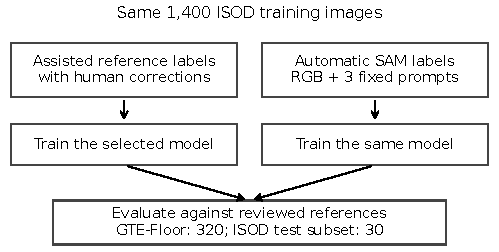
\includegraphics[width=\columnwidth]{figures/supervision_pipeline.pdf}
\caption{Comparison of reference and automatic training labels. The same model is trained on the same images with each set of labels. Both trained models and SAM 3's own masks are evaluated against reference test masks.}
\label{fig:pipeline}
\end{figure}

\begin{figure*}[!b]
\centering
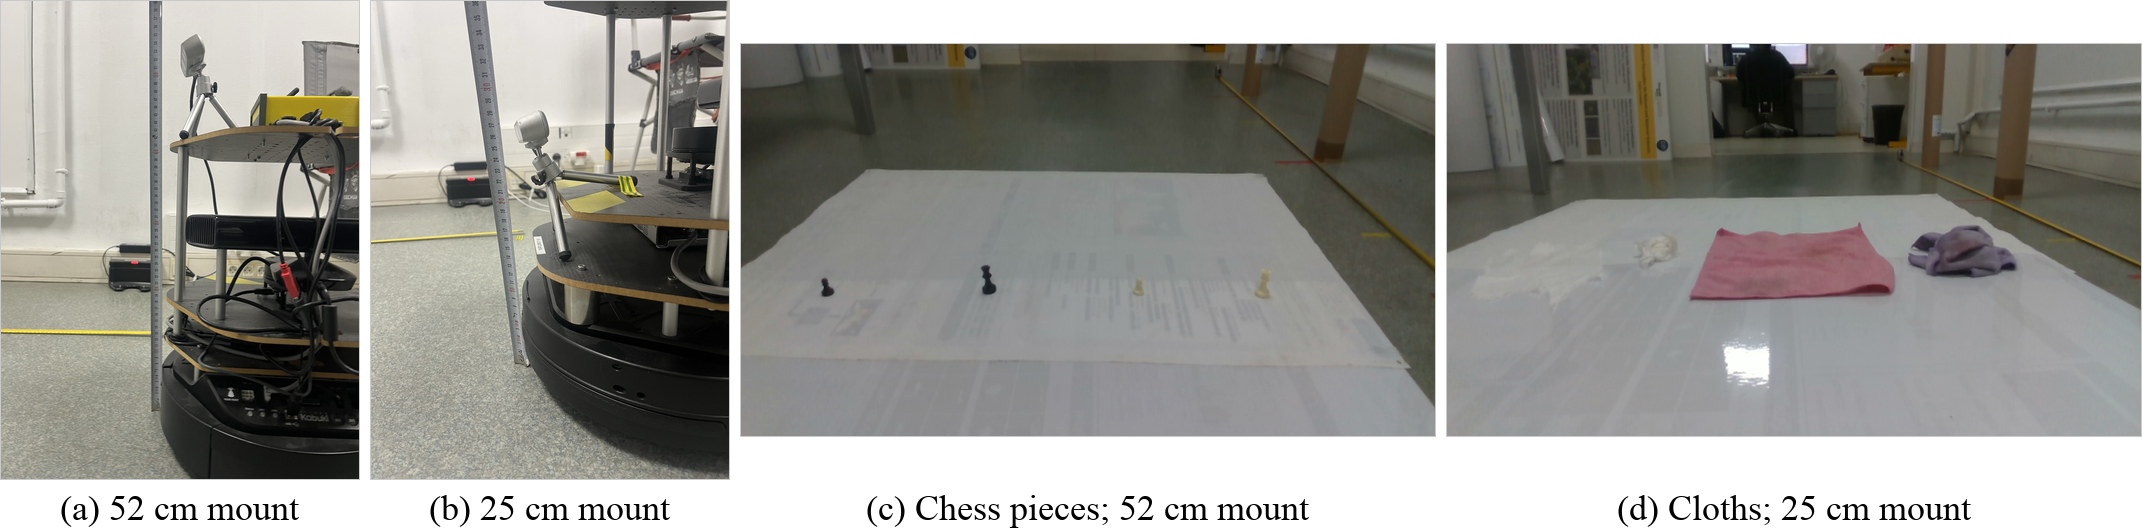
\includegraphics[width=\textwidth]{figures/collection.png}
\caption{RealSense D435 mounted at (a) 52 cm and (b) 25 cm. Example GTE-Floor images show (c) white/black chess pieces and (d) flat/crumpled cloths on a white poster, both at the 0.75 m floor mark. These objects differ in height and visibility against the background.}
\label{fig:collection}
\end{figure*}

\subsection{Datasets and reference
annotations}\label{datasets-and-reference-annotations}

\subsubsection{ISOD}\label{isod}

The Indoor Small Objects Dataset (ISOD) was introduced by Chen et
al.~\cite{chen2023self} to evaluate MOSTS for drivable-area
segmentation. We choose it for its paired RGB-D images and low-lying
floor objects. Its 2,000 images were captured at 20 recording locations
with a RealSense D455. We assign 14 locations to training, three to
validation and three to testing, giving 1,400/300/300 images. Each
location stays in one partition to prevent overlap between training and
test scenes.

ISOD provides drivable/not-drivable masks; the latter includes walls and
furniture as well as floor objects. We construct obstacle references
using SAM object/structure proposals constrained by the original
not-drivable mask, with floor-contact and connected-region rules to
recover missed fragments and reject structure. Human review corrects
inclusion errors, omissions and regions joined to furniture. These are
assisted reference labels, rather than a fully manually annotated
training set: the frozen 1,400 training masks contain 70 reviewed masks
and 1,330 assisted proposals. All 300 validation masks were reviewed.
The reported ISOD test scores use 30 reviewed frames, ten per test
location, rather than the full 300-frame test split. A subsequent
16-frame training review supplies the newer box-detector reference
version, with 85 reviewed and 1,315 assisted masks; semantic models keep
the frozen version above. Movable floor items are retained,
including larger controls; no measured height cutoff is imposed.

\subsubsection{GTE-Floor}\label{gte-floor}

We collected GTE-Floor in the GTE campus laboratory using a RealSense
D435 on a TurtleBot. Its 64 static-scene recordings contain five images
each (320 images), used only for external evaluation of models trained
on ISOD. The seven object sets include thin, flat and taller objects,
with pale and dark items to vary visibility. Table \ref{tab:collection}
lists the collection conditions; Fig. \ref{fig:collection} shows the
mounts and examples, and the appendix shows the object sets. We
initialize reference masks with SAM labels and refine them manually.
Figure~\ref{fig:objects} presents the object inventory. Object-type annotations let us compare how often cables and cloths are
detected, although both share one obstacle class.

\begin{table}[H]
\caption{GTE-Floor dataset composition}
\label{tab:collection}
\centering
\footnotesize
\begin{tabularx}{\columnwidth}{@{}>{\raggedright\arraybackslash}p{0.22\columnwidth}>{\raggedright\arraybackslash}Xr@{}}
\toprule
Background & Objects & Runs \\
\midrule
Floor & Cables, tape rolls, hex keys, mixed items, screws, chess, cloths/tissues; \mbox{reference (no objects)} & 44 \\
White poster & Cables, chess, cloths/tissues; \mbox{reference (no objects)} & 20 \\
\bottomrule
\end{tabularx}
\par\smallskip
\begin{minipage}{\columnwidth}
\footnotesize
Camera heights: 25 and 52 cm; floor distances: 0.75, 1.5 and 2.5 m. Reference scenes cover both heights and backgrounds.
\end{minipage}
\end{table}

\subsection{Models and training}\label{models-and-training}

We compare ESANet's RGB, D and RGB-D versions using the authors'
ResNet-34 NBt1D models \cite{seichter2021efficient}. The additional depth encoder also changes model capacity; the
comparison tests these ESANet configurations rather than isolating
input information at an identical parameter count.

To compare established methods for individual modalities, we also
evaluate U-Net and YOLOv8n-seg using RGB, and a geometric method using D
(Table \ref{tab:models}). The geometric method fits a floor plane to
detect objects protruding from the floor.

\begin{table}[H]
\caption{Methods compared for small floor-obstacle detection}
\label{tab:models}
\centering
\footnotesize
\begin{tabularx}{\columnwidth}{@{}l*{3}{>{\centering\arraybackslash}X}@{}}
\toprule
Method & RGB & D & RGB-D \\
\midrule
ESANet & Yes & Yes & Yes \\
U-Net & Yes & -- & -- \\
YOLOv8n-seg & Yes & -- & -- \\
YOLOv8n detector & Yes & -- & -- \\
Floor-plane fit & -- & Yes & -- \\
\bottomrule
\end{tabularx}

\end{table}

We follow the ESANet authors' preprocessing and weight initialization.
RGB images use the normalization required by the pretrained encoder.
Depth values are normalized using the mean and standard deviation of
valid readings from ISOD training images; these same values are used on
GTE-Floor. Missing depth readings follow the authors' raw-depth
preprocessing.

ESANet uses \(640\times448\) inputs, batch size 8, SGD with learning
rate 0.01, momentum 0.9, weight decay \(10^{-4}\) and a OneCycle
learning-rate schedule. Class weights account for the imbalance between
obstacle and background pixels using the authors' median-frequency
method. We train for 500 epochs, following the published training
duration, and select the checkpoint with the best validation obstacle
IoU. Learning curves are checked for convergence before comparing input
types.

U-Net uses an ImageNet-pretrained MobileNetV2 encoder, batch size 8,
AdamW with learning rate \(3\times10^{-4}\) and cross-entropy plus soft
Dice loss. YOLOv8n-seg uses pretrained RGB weights, 640-pixel inputs and
batch size 16. For YOLO, training masks are converted to polygons; its
predicted object masks are combined for evaluation.
U-Net runs for 15 epochs and YOLO for 20; checkpoints are selected by
reference-validation obstacle IoU.

The separate YOLOv8n box detector uses COCO-pretrained weights,
640-pixel inputs, batch size 16 and SGD for 20 epochs, with three matched
seeds per label source. One reference-instance ID becomes one enclosing
box, including disconnected visible parts. Shared 300-frame reference
validation boxes select the best checkpoint by box AP50:95. Instance
targets are assisted proposals and include unresolved groups.

\subsection{Automatic labeling}\label{automatic-labeling}

We test whether automatic labeling with SAM 3 can reduce manual
annotation without reducing obstacle-detection performance. We measure
the accuracy of its masks and the performance of models trained on them
without human correction.

The automatic teacher is separate from reference construction. SAM 3
receives the full RGB image and the fixed prompts ``small object on the
floor'', ``cable on the floor'' and ``things on the floor''. Masks with
confidence at least 0.6 are combined by union, with mask-probability
threshold 0.5. Generation uses no ISOD masks, human reference masks,
negative prompts or per-image corrections. Prompt development used 30
reviewed training frames, followed by validation-informed ablation on
the 300 reviewed validation frames; this is therefore not an
annotation-free end-to-end procedure. The checkpoint and prompts remain
fixed for every generated image, including empty scenes.

The completed ESANet runs compare these automatic masks with the frozen
reference training masks. Automatic masks are used without human
correction, including empty predictions and labeling failures. Completed
U-Net and YOLOv8n-seg reference runs provide additional RGB comparisons.
For automatic box-detector targets, fresh SAM instance predictions from
the same three prompts undergo mask-overlap duplicate and parent/child
resolution before box conversion, without reference-mask input.

Both training sets label the full image as obstacle or background.

\subsection{Evaluation}\label{evaluation}

We evaluate SAM 3's masks and all methods in Table \ref{tab:models}
against reference test masks from ISOD and GTE-Floor. We report pooled pixel IoU as a companion measure of mask quality. GTE-Floor results are grouped by object type, pixel size, nominal floor
distance, camera setup and background. Coverage recall counts reference units with at least half their pixels
predicted. We interpret this alongside false components and reference-unit
localization: the union of touching predicted components must achieve
adjusted IoU of at least 0.5, retaining their extra background extent
while excluding other annotated targets from that background penalty.
A prediction covering the whole poster therefore does not establish
localization of its small targets. Reference IDs include explicit object
groups; this diagnostic is not native instance AP. Full-frame false
components include recording props and are not a clean estimate of
operational false alarms. Five static repeats are averaged within
recordings for condition summaries; error bars show variation across
training seeds, not independent-scene confidence intervals.

\clearpage
\section{Results and Discussion}\label{sec:results}

\begin{figure*}[!b]
\centering
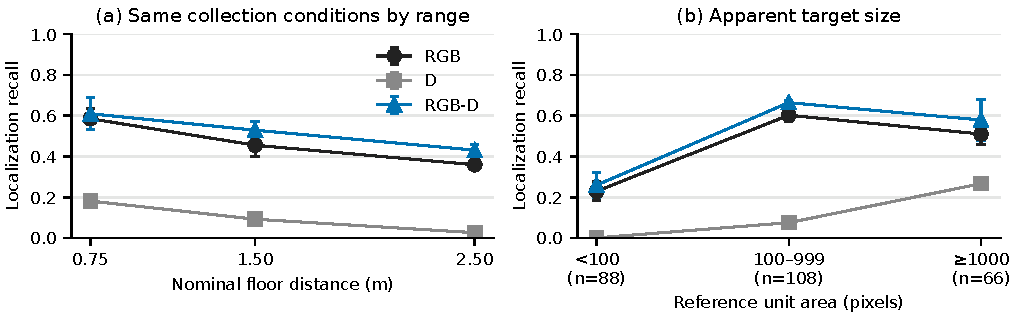
\includegraphics[width=\textwidth]{figures/range_and_size.pdf}
\caption{ESANet reference-supervised localization by (a) nominal floor distance and (b) reference-mask area. Points show three-seed means; bars show seed standard deviation, not independent-scene confidence intervals. Panel (a) averages the five static repeats within each of 20 recordings per distance. Panel (b) averages repeats within reference-unit/recording pairs; $n$ includes explicit object groups. Pixel size, category and distance covary. All predictions use full images; recording props remain in the diagnostic domain.}
\label{fig:range-size}
\end{figure*}

\subsection{Experimental comparisons}

We evaluate the completed runs on all 320 GTE-Floor frames, without
fine-tuning on these recordings. Table~\ref{tab:results} reports the
reference-supervised comparators and the accepted three-prompt SAM
supervision. ESANet uses three seeds per condition, except automatic
RGB, for which two completed seeds are available. Supervision changes
are compared using matching seeds only. Historical SAM-label versions
are excluded from this comparison. The RGB-D repeats use the same
PyTorch 2.10 version as the RGB and D experiments.

\begin{table}[H]
\caption{GTE-Floor diagnostic results. IoU and recalls are percentages. IoU and localization recall $R_{\mathrm{loc}}$ (adjusted IoU $\geq0.5$) show mean $\pm$ seed standard deviation. Coverage recall $R_{\mathrm{cov}}$ (at least half the target covered) and false components/frame (FC) show means. $n$ counts seeds; direct methods are fixed. Full frames include props, with no area filter. SAM uses the three-prompt labels.}
\label{tab:results}
\centering
\footnotesize
\setlength{\tabcolsep}{2.5pt}
\begin{tabular}{@{}lrcccc@{}}
\toprule
Model / labels & $n$ & IoU & $R_{\mathrm{cov}}$ & $R_{\mathrm{loc}}$ & FC \\
\midrule
RGB / reference & 3 & 48.6 $\pm$ 7.5 & 62.8 & 45.4 $\pm$ 1.8 & 3.65 \\
D / reference & 3 & 14.1 $\pm$ 1.2 & 38.3 & 9.8 $\pm$ 1.2 & 8.24 \\
RGB-D / reference & 3 & 55.4 $\pm$ 8.8 & 64.3 & 50.7 $\pm$ 4.6 & 2.84 \\
RGB / SAM & 2 & 46.8 $\pm$ 3.0 & 75.2 & 60.1 $\pm$ 0.2 & 5.76 \\
D / SAM & 3 & 12.6 $\pm$ 1.8 & 36.3 & 9.7 $\pm$ 2.0 & 8.82 \\
RGB-D / SAM & 3 & 49.8 $\pm$ 3.7 & 75.3 & 60.7 $\pm$ 1.6 & 6.03 \\
U-Net / reference & 3 & 48.5 $\pm$ 1.5 & 52.0 & 44.4 $\pm$ 1.5 & 3.18 \\
YOLO / reference & 3 & 45.9 $\pm$ 1.0 & 60.0 & 47.1 $\pm$ 3.3 & 1.01 \\
Direct SAM & -- & 41.8 & 94.5 & 84.0 & 2.54 \\
Floor fit & -- & 3.8 & 69.5 & 5.7 & 344.02 \\
\bottomrule
\end{tabular}
\end{table}

\subsection{Contribution of depth and object scale}

Reference-supervised RGB-D reaches mean GTE-Floor IoU 0.554, compared
with 0.486 for RGB and 0.141 for D. The paired RGB-D minus RGB IoU
changes range from $-6.3$ to $+20.3$ percentage points across seeds;
the mean gain of 6.8 points is therefore not consistent across runs.
Localization recall increases from 0.454 to 0.507, while coverage recall
changes only from 0.629 to 0.643: tighter localization is not necessarily
a newly recovered object. The mean localization advantage persists at
overlap thresholds 0.25, 0.50 and 0.75 (4.2, 5.3 and 5.8 points).
U-Net and YOLO provide comparable RGB results, with different
localization/false-component tradeoffs (Table~\ref{tab:results}).
On the limited 30-frame reviewed ISOD test subset, RGB and RGB-D mean
IoU are 0.754 and 0.753; these provisional scores do not establish a
fusion advantage on the full test split.

In Fig.~\ref{fig:range-size}(a), mean recording-level localization
recall falls from 0.585 to 0.359 for RGB between the 0.75 and 2.5 m
marks, from 0.610 to 0.431 for RGB-D, and from 0.181 to 0.026 for D.
Small apparent targets are also difficult to localize (Fig.~\ref{fig:range-size}(b)).
The observations support a range/scale limitation, but distance changes
pixel area and viewpoint together; they do not isolate depth noise.

\begin{figure*}[!t]
\centering
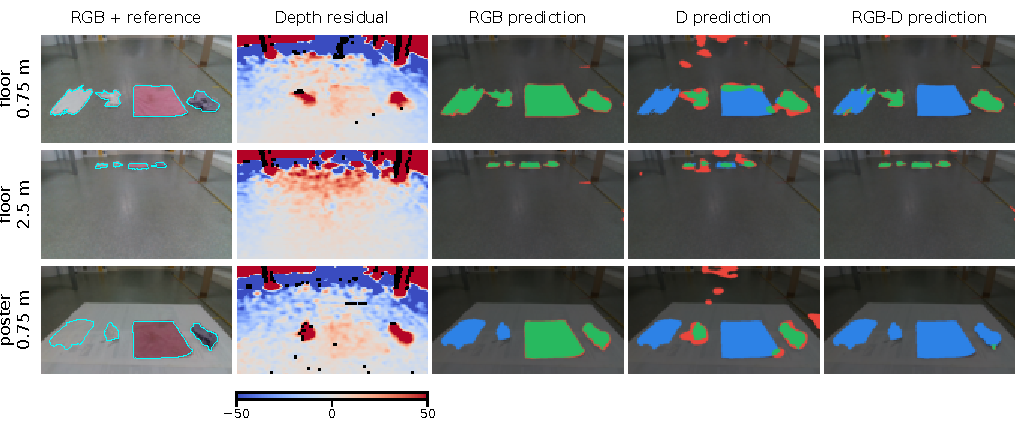
\includegraphics[width=\textwidth]{figures/cloth_depth_examples.pdf}
\caption{Matched cloth/tissue views: near/far bare floor and the near white poster, using the 52 cm camera configuration, frame 2 and seed 0. All rows retain the same full-image scale. Cyan outlines show the reference; prediction colors are green for correct foreground, blue for missed foreground and red for extra foreground. Residuals share a $[-50,50]$ mm scale; black marks unavailable values. This camera-axis floor-fit residual is not physical height. The leftmost flat towel has little positive near residual, unlike the adjacent crumpled tissue. Fusion misses flat foreground in the near floor view despite RGB success; neither model rescues the flat white towel on the poster.}
\label{fig:cloth-depth}
\end{figure*}

\subsection{Qualitative evidence and depth reliance}

Figure~\ref{fig:cloth-depth} illustrates why valid depth is not the
same as a useful obstacle cue. At the near mark, median valid-depth
fractions exceed 0.99 for both the flat paper towel and crumpled tissue,
but their median object-versus-nearby-floor residual differences are
approximately $-0.8$ and $+43.5$ mm. Across all seeds and repeats, D
localizes the near crumpled tissue but misses the flat towel at all
three marks. RGB localizes both throughout; RGB-D misses the near towel
in one seed. This is descriptive, not a controlled folding experiment:
the items differ in material, shape and area.

In matched floor/poster recordings, the flat white towel is missed on
the poster by both RGB and RGB-D across all seeds and repeats, despite
frequent localization on bare floor. Its nearby-floor color difference
also decreases. This is a difficult low-contrast case, not evidence that
depth compensates for missing RGB contrast; background context changes
alongside appearance.

Keeping RGB and model weights fixed, replacing depth with missing
readings reduces mean RGB-D IoU from 0.554 to 0.147. However, permuting
depth between object sets within the same camera/background/distance
configuration gives 0.547. Missing depth is an out-of-distribution
input, while the permutation preserves much scene geometry. Thus the
zero-depth degradation alone does not demonstrate use of precise
object-level depth; these checks measure reliance under interventions.

\subsection{Automatic supervision and limitations}

For RGB-D, replacing reference training masks with the RGB-only SAM
labels changes mean IoU from 0.554 to 0.498, but raises localization
recall from 0.507 to 0.607, coverage recall from 0.643 to 0.753, and
false components from 2.84 to 6.03 per frame. The gain in recovered reference units is accompanied by more
excess detections, rather than an unqualified improvement. RGB shows
the same recall/false-component tradeoff on its two matched seeds;
D remains weak with either supervision. Direct SAM localizes 0.840 of
reference units but reaches only 0.418 pixel IoU. Detection and boundary
accuracy therefore require separate reporting.

Teacher-mask pooled IoU is 0.604 on 300 reviewed validation frames and
0.757 on 30 reviewed test frames. Validation informed prompt selection,
so its quality estimate is not independent. A retrospective 370-frame
reference-assistance replay gives mean image IoU 0.878; a later 14-frame
random check gives 0.837 with two major errors. Both reference assistance
and the teacher use SAM, so correlated annotation errors can remain
after review. GTE-Floor covers one room; camera height and tilt change
together. Grouped references and recording props limit the full-frame
diagnostic; it is not operational accuracy or instance AP.

\section{Conclusion and Future Work}\label{sec:conclusion}

RGB appearance provides a strong floor-obstacle baseline. RGB-D improves
average external localization and IoU, but its gain varies across seeds
and is not supported by every object example. Depth alone struggles
with small, flat and distant targets. Automatic SAM labels can train
models that recover more reference units, with a substantial
false-component cost. Future work should expand reviewed ISOD test
coverage, verify instance/group annotations, and evaluate fixed
collection-area crops with recording props handled explicitly. Those
steps are needed before claiming reliable individual-object detection
or deployment performance.

\clearpage

\IEEEtriggeratref{8}
\bibliographystyle{IEEEtran}
\bibliography{refs}

\onecolumn

\appendix[GTE-Floor Object Sets]\label{app:objects}

\begin{figure}[H]
\centering
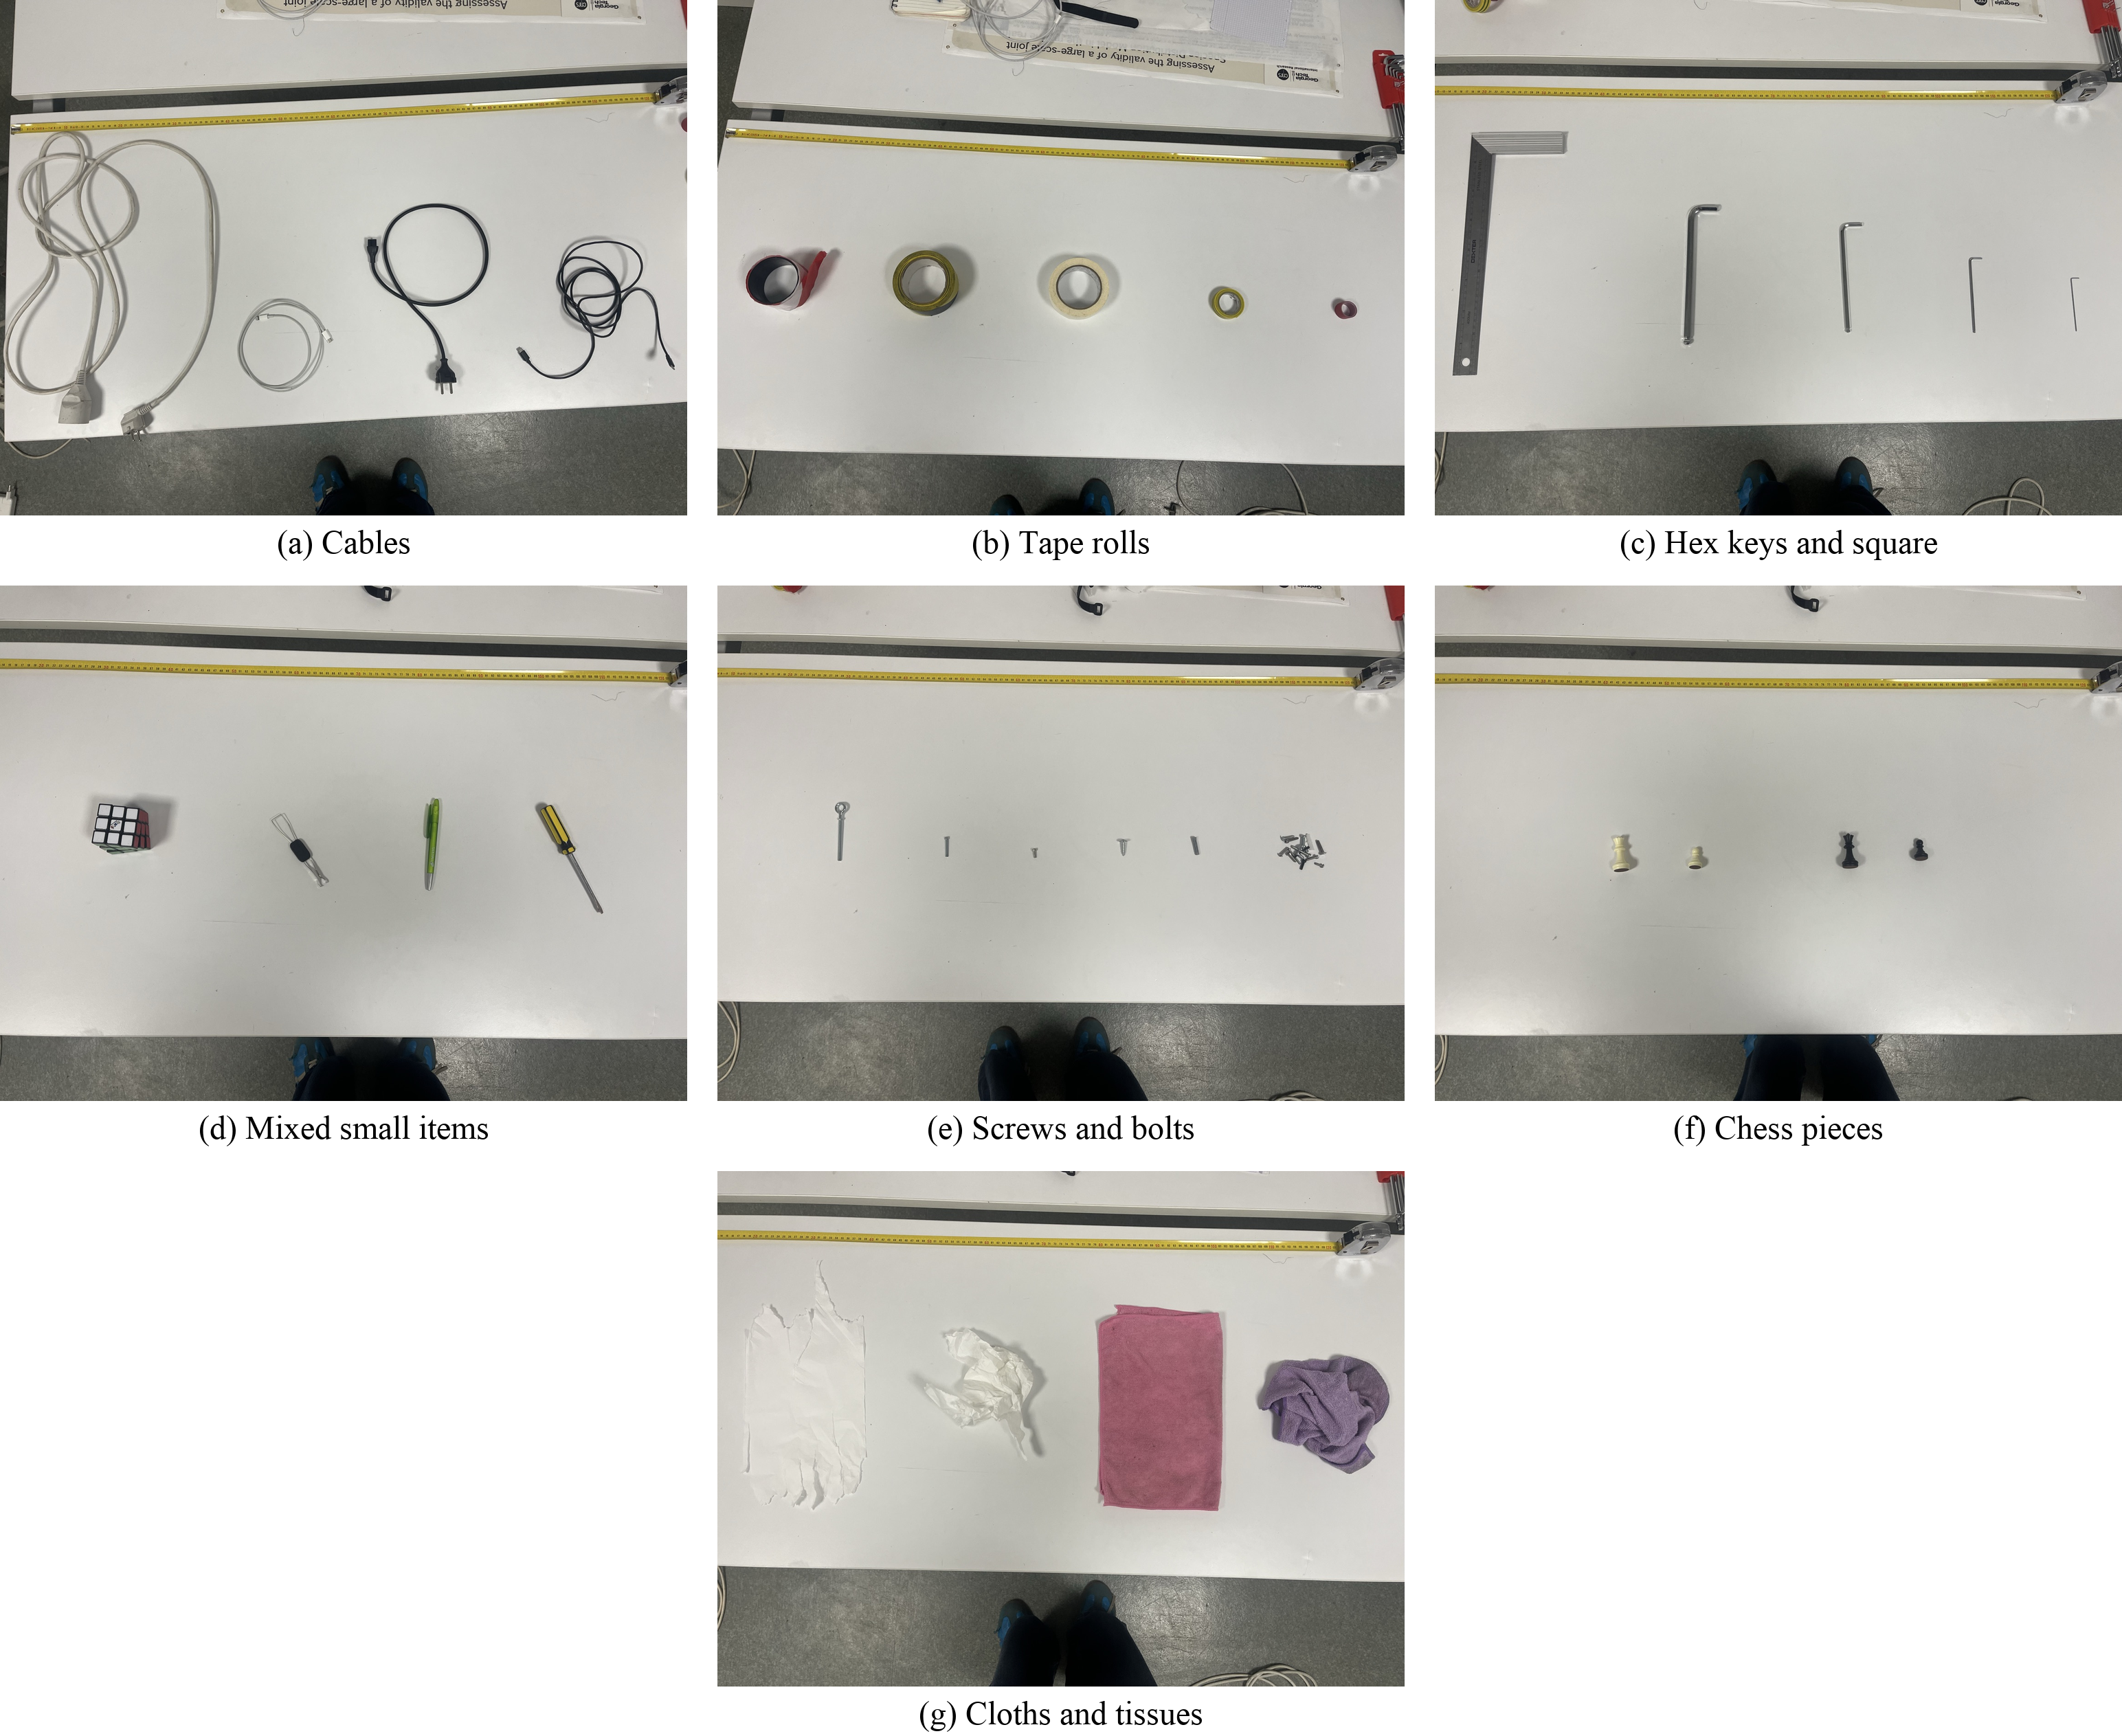
\includegraphics[width=\textwidth,height=0.75\textheight,keepaspectratio]{figures/object_sets.png}
\caption{GTE-Floor's seven object sets. Cables, hex keys and screws provide thin or small obstacles; cloths and tissues include flat and crumpled forms. Tape rolls and chess pieces provide taller objects, while the mixed set adds everyday items.}
\label{fig:objects}
\end{figure}

\end{document}
